\documentclass{standalone}
\usepackage{tikz}

\begin{document}

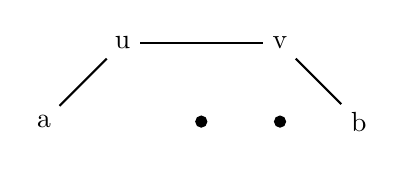
\begin{tikzpicture}[node distance=1cm]

    % Nodes
    \node (u) at (0,0) {u};
    \node (v) at (2,0) {v};
    \node (a) at (-1,-1) {a};
    \node (b) at (3,-1) {b};

    % Edges
    \draw[thick] (u) -- (v);
    \draw[thick] (u) -- (a);
    \draw[thick] (v) -- (b);

    % Dots for second neighborhood
    \filldraw[black] (1,-1) circle (2pt); % Center dot between u and v
    \filldraw[black] (2,-1) circle (2pt); % Dot for v

\end{tikzpicture}

\end{document}